\documentclass[tikz, dvisvgm]{standalone}
\usepackage{pgfplots}
\pgfplotsset{compat=1.18}

\begin{document}
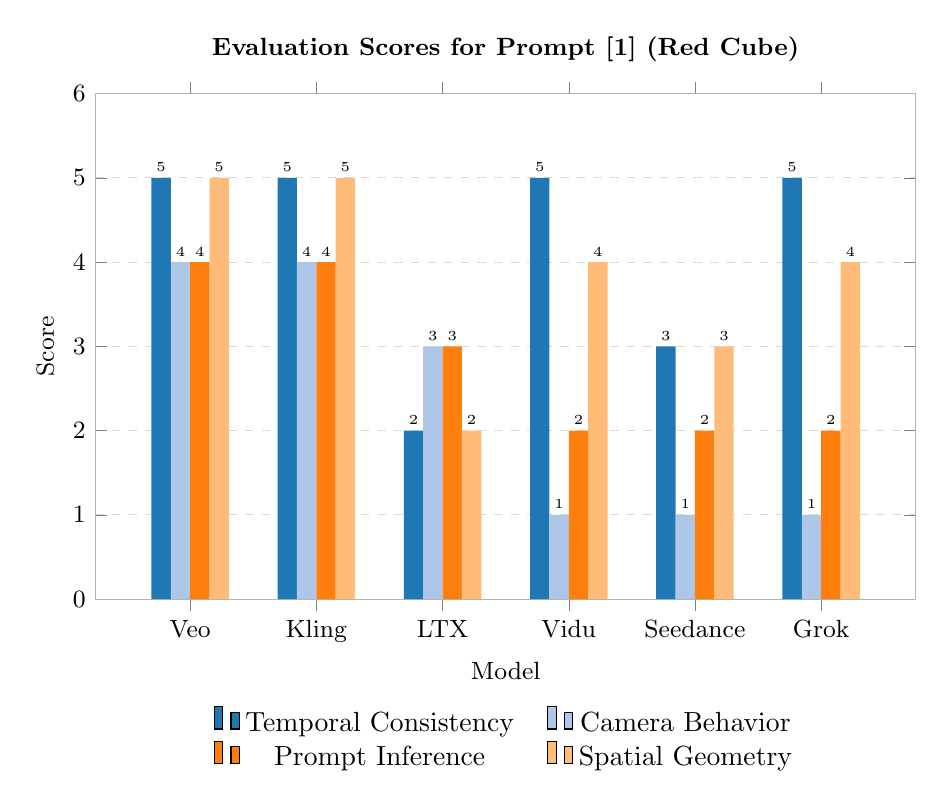
\begin{tikzpicture}
    % Define the professional color palette
    \definecolor{color1}{RGB}{31, 119, 180}
    \definecolor{color2}{RGB}{174, 199, 232}
    \definecolor{color3}{RGB}{255, 127, 14}
    \definecolor{color4}{RGB}{255, 187, 120}

    \begin{axis}[
            ybar=0pt,
            bar width=7pt,
            width=12cm, % Use a fixed width for SVG export
            height=8cm,  % Use a fixed height for SVG export
            symbolic x coords={Veo, Kling, LTX, Vidu, Seedance, Grok},
            xtick=data,
            ymin=0, ymax=6,
            ylabel={Score},
            xlabel={Model},
            title={Evaluation Scores for Prompt [1] (Red Cube)},
            ymajorgrids=true,
            grid style={dashed, gray!30},
            axis line style={gray!60},
            legend style={
                at={(0.5,-0.2)}, 
                anchor=north, 
                legend columns=2, 
                draw=none,
                /tikz/every even column/.append style={column sep=10pt}
            },
            nodes near coords,
            every node near coord/.append style={font=\tiny, inner sep=2pt},
            label style={font=\small},
            tick label style={font=\small},
            title style={font=\bfseries\small, yshift=2pt},
            enlarge x limits=0.15,
        ]
        
        \addplot[fill=color1, draw=none] coordinates {
            (Veo,5) (Kling,5) (LTX,2) (Vidu,5) (Seedance,3) (Grok,5)
        };
        
        \addplot[fill=color2, draw=none] coordinates {
            (Veo,4) (Kling,4) (LTX,3) (Vidu,1) (Seedance,1) (Grok,1)
        };
        
        \addplot[fill=color3, draw=none] coordinates {
            (Veo,4) (Kling,4) (LTX,3) (Vidu,2) (Seedance,2) (Grok,2)
        };
        
        \addplot[fill=color4, draw=none] coordinates {
            (Veo,5) (Kling,5) (LTX,2) (Vidu,4) (Seedance,3) (Grok,4)
        };

        \legend{Temporal Consistency, Camera Behavior, Prompt Inference, Spatial Geometry}
    \end{axis}
\end{tikzpicture}
\end{document}